\onehalfspacing

\section{Open Science}

Was das Schlüsselwort ,,Open'' im Kontext von Wissenschaft bedeutet, erschließt sich nicht sofort. Um also Open Science zu verstehen und warum diese als notwendig für die traditionelle Wissenschaft gewertet wird, wird die gleichnamige Bewegung in den Blick genommen und deren Ursprünge überblickt.\footnote{Genau genommen ist das Konzept von Open Science, also im Kern eigene Forschungsmethoden,  -praktiken und -ergebnisse transparent für andere zu machen, schon älter und findet Anwendung bereits in der Renaissance. Für das Thema dieser Arbeit ist eine longue durée letztlich wissenschaftlicher Praxis jedoch nicht relevant. Daher wird sich auf die aktuelle Bewegung und deren direkte Ursprünge begrenzt. Siehe auch Paul A. David: Common Agency Contracting and the Emergence of ,,Open Science'' Institutions, in: The American Economic Review (Hrsg.), 2. Ausgabe, 1998, S. 15–21, URL (stable): \url{http://www.jstor.org/stable/116885.}.} Zudem wird der Versuch unternommen, den Begriff Open Science für eine Anwendung in dieser Arbeit zu definieren. Anhand gegenwärtig existierender Konzepte und Infrastruktuen wird abschließend herausgearbeitet, wo Open Science steht. Daraus ergeben sich wiederum Konsequenzen für das offene Forschungsdatenmanagement. 

\subsection{Ursprünge der Open Science-Bewegung}

Die Entstehung der Open Science-Bewegung lässt sich anhand von zwei Entwicklungssträngen verfolgen. Zum einen geht sie auf ein konkretes Ereignis innerhalb der Wissenschaft zurück, das als Replikationskrise bzeichnet wird. Hier bezieht sich Open Science explizit auf die Transformation wissenschaftlicher Forschungsmethoden und -praktiken, um Forschung noch robuster zu machen. Zum anderen ist Open Science Teil der breiteren sozialen Open-Bewegung, welche von der Do-it-yourself-Bewegung, der Hacker-Bewegung der 1960/ 70er sowie der Freie-Software-Bewegung der 1980er Jahre
(Vorgänger der Open Source-Bewegung) beeinflusst ist.\footnote{Vgl. ayway media (Hrsg.): Das digitale Handbuch,
Kapitel C.15 Die ,,Open-Bewegung'', Vettelschloss 2016, S. 252}

\paragraph{Replikationskrise} Ab Mitte der 2010er Jahre erhielten in der Wissenschaft, vordergründig in der Psychologie sowie in den Lebens- und Naturwissenschaften, zunehmend Replikationsstudien Aufmerksamkeit. Diese konnten in sogenannten Replikationsversuchen eine statistisch signifikante Anzahl publizierter empirischer Forschungsergebnisse entweder falsifizieren oder nicht replizieren, weil die Daten nicht zur Verfügung standen.\footnote{Als erste Replikationsstudie dieser Art wird jene des Medizinwissenschaftlers und Statistiskers John Ioannidis aus dem Jahr 2005 gezählt, mit der er erstmals systematisch versuchte, veröffentlichte Untersuchungsergebnisse nachträglich zu replizieren/ reproduzieren. Siehe John P.A. Ioannidis: Why Most Published Research Findings Are False, PLoS Med 2(8): e124, 2005, doi:10.1371/journal.pmed.0020124. Es folgten eine Reihe weiterer Replikationsstudien auch in anderen Fächern wie den Sozialwissenschaften. Siehe zum Beispiel Marjan Bakker, Annette van Dijk, Jelte M. Wicherts: The Rules of the Game Called Psychological Science, in: Perspectives on Psychological Science, 7(6), 2012, S. 543-554, doi:10.1177/1745691612459060; Thomas Herndon, Michael Ash, Robert Pollin: Does high public debt consistently stifle economic growth? A critique of Reinhart and Rogoff, in: Cambridge Political Economy Society (Hrsg.), Cambridge Journal of Economics, Band 38, 2. Ausgabe, Oxford 2014, S. 257-279, URL (stable): \url{https://www.jstor.org/stable/24694929}; Jeremy Freese, David Peterson: Replication in Social Science, in: Annual Reviews (Hrsg), Annual Review of Sociology, Band 43, San Mateo 2017, S. 147-165, doi:10.1146/annurev-soc-060116-053450} Das löste die vielfach diskutierte ,,Replikationskrise'' in den betroffenen Fächern aus. Zum einen ging es, bezüglich der Falsifizierungen, nachträglich um Ursachenforschung, die sich auf Defizite insbesondere bei den Forschungsmethoden und in der Publikationspraxis wissenschaftlicher Journals konzentrierte.\footnote{Diskutiert wurden insbesondere, wie das Institut für Psychologie an der Humboldt-Universität zu Berlin konzis berichtete, "p-hacking, selektives Berichten von (abhängigen) Variablen, Hypothesizing After the Results are Known (HARKING), nur signifikante Ergebnisse berichten, mehr Daten sammeln nachdem die bestehenden Daten keine positiven Ergebnisse hervorgebracht haben, Publikations Bias". Methodengruppe Berlin (Autorengruppe): Die Replikationskrise und Open Science, Blog Post, Humboldt-Universität zu Berlin, Lebenswissenschaftliche Fakultät Institut für Psychologie, Lehrstuhl für Psychologische Methodenlehre (Hrsg), URL: \url{http://methods-berlin.com/de/replikationskrise_open_science/} (letzter Zugriff am 21.04.2022). Siehe auch Klaus Fiedler, Norbert Schwarz: Questionable Research Practices Revisited, in: SAGE Publishing (Hrsg.), Social Psychological and Personality Science, Band 7, 1. Ausgabe, 2016, S. 45-52, doi:10.1177/1948550615612150; Annie Franco, Neil Malhotra, Gabor Simonovits: Publication bias in the social sciences. Unlocking the file drawer, in: American Association for the Advancement of Science (Hrsg.), Science, Band 345, Ausgabe 6203, Washington 2014, S. 1502-1505, doi:10.1126/science.1255484.} Aber auch die Replikationsstudien selbst wurden kritisch betrachtet.\footnote{Vgl. Deutsche Forschungsgemeinschaft (Hrsg.): Replizierbarkeit von Forschungsergebnissen. Eine Stellungnahme der Deutschen Forschungsgemeinschaft, Stand: April 2017, URL: \url{https://www.dfg.de/download/pdf/dfg_im_profil/geschaeftsstelle/publikationen/stellungnahmen_papiere/2017/170425_stellungnahme_replizierbarkeit_forschungsergebnisse_de.pdf} (letzter Zugriff am 21.04.2022).} Zum anderen war, bezüglich der Nichverfügbarkeit von Daten, eine wesentliche Eigenschaft von robuster evidenzbasierter Forschung, nämlich die Nachvollziehbarkeit ihrer Ergebnisse durch Replikation (als Bestandteil von Qualitätssicherung), nicht mehr gegeben und damit in der Konsequenz auch ein gesellschaftlicher Bedeutungsverlust von Wissenschaft bei der Wissensproduktion zu befürchten. 

Kurzum ging es um die existenzielle Frage, wie Wissenschaft praktiziert werden muss, damit wissenschaftliche Forschung, insbesondere die statistisch empirische, reliabel ist. Als Antwort auf diese Krise hat sich in den vergangenen Jahren die internationale Open Science-Bewegung formiert\footnote{Entsprechend der Internationalität der Open Science-Bewegung, existieren weltweit Open Science Initiativen, von denen allein in Deutschland hier nur eine Auswahl wiedergegeben werden kann: Berlin School of Public Engagement and Open Science als Kollaborationsprojekts des Museums für Naturkunde Berlin, der Humboldt-Universität zu Berlin und der Robert-Bosch-Stiftung, URL: \url{https://www.museumfuernaturkunde.berlin/de/future/wissenschaftscampus/berlin-school-public-engagement-and-open-science}; Open Science Working Group an der FU Berlin, URL: \url{https://www.fu-berlin.de/sites/open-science}; Open Science Center an der LMU München;  Initiative für Offene Wissenschaft und Innovation des Stifterverbands, URL: \url{https://www.stifterverband.org/open-science-innovation-netzwerke}.}, die in den Anfangsjahren stark auf die Frage nach Replizierbarkeit von Forschungsstudien fokussiert war. 

In Deutschland hat sich zuletzt das \textit{German Reproducibility Network} (GRN) gegründet, das fachübergreifend gezielt Replikationsstudien und Open Science-Praktiken unterstützen möchte.\footnote{Zu dessen Hauptakteuren gehören u.a. Berlin University Alliance, das Helmholtz Center (Open Science), das LMU Open Science Center (OSC), das Netzwerk der Open Science Initiativen (NOSI), die Deutsche Gesellschaft für Psychologie (DGPs), u.a. Siehe Ankündigung der Berlin University Alliance: German Reproducibility Network gestartet, News vom 01.02.2021, URL: \url{https://www.berlin-university-alliance.de/news/items/2021/210201-grn.html}. Homepage des GRN unter URL: \url{https://reproducibilitynetwork.de/} (alle letzter Zugriff am 27.04.2022).} Auf internationaler Ebene ist vor allem das interdisziplinäre \textit{Center for Open Science} (COS) zu nennen, welches in direkter Reaktion auf die Replikationskrise 2013 in den USA gegründet worden war.\footnote{URL: \url{https://www.cos.io/?hsLang=en} (letzter Zugriff am 21.04.2022).} Eine der ersten Aktivitäten des COS war das mit der University of Viginia gemeinsam großangelegte \textit{Reproducibility Project}, in dem sich eine Autorengruppe, welche sich ,,Open Science Collaboration'' nannte, systematisch mit der Reproduzierbarkeit von 100 Forschungsstudien in der Psychologie auseinandersetzte.\footnote{Brian A. Nosek, Johanna Cohoon, Mallory C. Kidwell, Jeffrey R. Spies: Estimating the reproducibility of psychological science, in: American Association for the Advancement of Science (Hrsg.), Science, Band 349, Ausgabe 6251, Washington 2015, doi:10.1126/science.aac4716.}. Nach einer Bestandsaufnahme, bei der die Rate nichtreplizierbarer Forschungsstudien wie bei vorausgegangenen Replikationsstudien signifikant hoch war, widmete sich das COS verstärkt den Strategien zur Überwindung der Replikationskrise, die im Kern ebenfalls als eine methodische Krise identifiziert wurde sowie zweifelhafte Forschungspraktiken aufdeckte.

\paragraph{Open-Bewegung} Die Open Science-Bewegung ist Teil der breiten sozialen Open-Bewegung, welche unter den Begriffen ,,Open'', ,,Openness'' beziehungsweise ,,Free'' subsumiert, ,,Daten, Entwürfe, Fotos, Musikstücke oder sonstige Inhalte und Wissen'' \footnote{Wikimedia Deutschland e. V., Open Knowledge Foundation Deutschland e. V. (Hrsg.): ABC der Offenheit, Berlin 2019, S. 4f., URL: \url{https://commons.wikimedia.org/wiki/File:ABC_der_Offenheit_-_Broschüre_(2019).pdf} (letzter Zugriff am 26.04.2022).} aus allen gesellschaftlichen Bereichen zur Weiterverbreitung sowie Wiederverwendbarkeit schrankenlos zur Verfügung stellen und dadurch Teilhabe als demokratisches Prinzip in einer freiheitlichen Gesellschaft stärken will. Außerdem sieht sie in einer Kultur der Offenheit Potenzial für neue Innovationen.\footnote{Ebd. sowie siehe auch Open Knowledge Foundation (Hrsg.): Why open data? URl: \url{https://okfn.org/opendata/why-open-data/} (letzter Zugriff am 26.04.2022).} Diese Forderungen sind zwar nicht grundsätzlich neu, bekamen aber mit der Verbreitung des World Wide Web (WWW) ab Mitte der 1990er Jahre\footnote{Veröffentlichung des ersten Webbrowsers Netscape in offener Lizenz, die Personen auf der ganzen Welt mit PC und Internetverbindung ermöglichte, frei im Web ,,zu surfen''} einen neuen Schub. Dies ist in der Natur des WWW selbst begründet. Denn dessen Schlüsseleigenschaft ist es - seit seiner Entstehung 1989 - Informationen system- und plattformunabhängig in einer gemeinsamen Netzwerkinfrastruktur zu übertragen und auszutauschen.\footnote{Erfunden wurde das WWW vom Physiker und Informatiker Tim Berners-Lee, der 1989 am CERN in Genf arbeitete und technischen Lösungen suchte, wie unter Forschern schnell und einfach kommuniziert werden kann. Die grundlegenden Technologien des WWW waren und sind es bis heute: HTML zur Darstellung und Verlinkung von Informationen (Hyper Text Markup Language), URI/ URL (Unified Ressource Identifier bzw. Locator) zur Lokalisierung einer Ressource z.B. eines HTML-Dokuments im Rechnernetz, HTTP (Hyper Text Transfer Protocol) zur Übertragung dieser Ressource im Rechnernetz. Zur detaillierten Historie, Funktionsweise und weiteren Entwicklung des WWW siehe zum Beispiel Tim Berners-Lee, Mark Fischetti: Weaving the web. The original design and ultimative destiny of the World Wide Web by its inventor, New York 2011. Niels Brügger: Web history, New York, Bern 2010. James Gilles, Robert Cailliau: How the Web was born. The story of the World Wide Web, Oxford University Press, 2000.} Damit eignete es sich auch, die Forderungen der Open-Bewegung technisch umzusetzen. Folglich werden überwiegend webbasierte Technologien in der Open-Bewegung eingesetzt, insbesondere die des Web 2.0, welche die Interaktionsmöglichkeiten im digitalen Raum erheblich erweiterten.\footnote{Vgl. Benedikt Fecher, Sönke Friesike: Open Science. One Term, Five Schools of Thought, Springer, 2014, S.11, doi:10.1007/978-3-319-00026-8\_2.} Eine wichtige Voraussetzung für viele heutige Open (Science) Projekte war zudem, dass die Technologien hinter dem WWW selbst von Anfang an offen waren, diese also (kosten)frei zur Verfügung standen und genutzt werden konnten.\footnote{Der Begründer Tim Berners-Lee hat sich von Anfang dafür eingesetzt das WWW offen zu halten. Er gründete 2012 in London das gemeinnützige Open Data Institute (ODI) mit, wodurch er selbst ein (einflussreicher) Vertreter der Open-Bewegung geworden ist. URL: \url{https://theodi.org/} (letzter Zugriff am 27.04.2022).} 

Die Open Science-Bewegung kann in diesem Kontext als Weiterentwicklung der vor 20 Jahren gegründeten Open Access-Bewegung gesehen werden, in der sich Wissenschaftler*innen 2002/2003 zusammengeschlossen haben, um offenen Zugang zu wissenschaftlichen Forschungsergebnissen zu fördern.\footnote{Siehe Erklärung der ,,Budapest Open Access Initiative'' vom 14.02.2002, URL: \url{https://www.budapestopenaccessinitiative.org/read/} sowie ,,Berliner Erklärung über den offenen Zugang zu wissenschaftlichem Wissen'' vom 22. Oktober 2003, abgerufen auf der Website der Max Planck Gesellschaft, URL: \url{https://openaccess.mpg.de/Berliner-Erklaerung} (alle letzter Zugriff am 02.05.2022)} Daneben umfasst die Open-Bewegung unter anderem Open Knowledge, Open GLAM, Open Government, Open Design, Open Innovation, wobei es eine trennscharfe Abgrenzung nicht gibt. So lässt sich Open Data auch als Querschnittsbereich auffassen, der in andere Bereiche wie Open Science hineinreicht.\footnote{Vgl. Birgit Schmidt, Astrid Orth, Gwen Franck, Iryna Kuchma, Petr Knoth, José Carvalho: Stepping up Open Science Training for European Research, in: Publications (Hrsg), 2 Ausgabe, 2016, S. 3, doi:10.3390/publications4020016. Eine konzise Übersicht aller Bereiche siehe auch WMK, OKF (2019), ABC der Offenheit, S. 14-54} Eine Vertreterin der ersten Stunde der Open-Bewegung und die wohl populärste ist die gemeinnützige Wikimedia Foundation, Inc. (WMF)\footnote{URL: \url{https://wikimediafoundation.org/de/} (letzter Zugriff am 22.04.2022)} mit Sitz in den USA.\footnote{Vgl. den Wikipedia-Eintrag zur Wikimedia Foundation, Seite ,,Wikimedia Foundation''. In: Wikipedia – Die freie Enzyklopädie. Bearbeitungsstand: 31. März 2022, 20:07 UTC. URL: \url{https://de.wikipedia.org/w/index.php?title=Wikimedia_Foundation\&oldid=221669459.} (letzter Zugriff am 22.04.2022) In Deutschland vertreten durch den Verein Wikimedia Deutschland e. V., vgl. ebd.} Bereits seit 2001 stellt sie digitale Dienste kostenfrei zur Verfügung, mit denen Wissen offen ausgetauscht und geteilt werden kann. Ihr bekanntestes und ältestes Projekt ist die freie Enzyklopädie \textit{Wikipedia}\footnote{URL: \url{https://de.wikipedia.org/wiki/Wikipedia:Hauptseite} (letzter Zugriff am 22.04.2022)}. Die WMF engagiert sich aber nicht ausschließlich mit der Wikipedia in der Open-Bewegung, sondern hat inzwischen eine Vielzahl an digitalen ,,Schwesternprojekten''.\footnote{Zum Beispiel das Wörterbuch Wictionary (2002), URL: \url{https://de.wiktionary.org/}; die Text- und Quellensammlung Wikisource (2003), URL: \url{https://de.wikisource.org/wiki/Hauptseite}; die Mediensammlung Wikimedia Commons (2004), URL: \url{https://commons.wikimedia.org/wiki/Hauptseite}; die Wissensdatenbank Wikidata (2012), URL: \url{https://www.wikidata.org/wiki/Wikidata:Main_Page} (alle letzter Zugriff am 22.04.2022). Eine Auflistung aller Wikimedia-Projekte ist auf der Homepage zu finden unter \url{https://www.wikimedia.de/projekte/} (letzter Zugriff am 22.04.2022)} Daneben stellt sie eine Reihe ihrer MediaWiki Software-Komponenten in Open Source zur Verfügung.\footnote{Eine Übersicht ist auf der Website zu finden unter URL: \url{https://doc.wikimedia.org/} (letzter Zugriff am 22.04.2022)} Eine weitere und mit der WMF koopierende Organisation in der Open-Bewegung ist die Open Knowledge Foundation (OKF), die 2005 in London gegründete wurde\footnote{URL: \url{https://okfn.org/} (letzter Zugriff am 22.04.2022).} und von der es seit 2011 auch einen deutschen Ableger in Berlin gibt.\footnote{URL: \url{https://okfn.de/} (letzter Zugriff am 22.04.2022).} Die OKF hat unter anderem das Open Source-Datenmanagementsystem \textit{ckan}\footnote{URL: \url{https://ckan.org/}. GitHub URL: \url{https://github.com/ckan/ckan} (alle letzter Zugriff am 15.05.2022).} entwickelt, mit dem Datenkollektionen verwaltet und als Open Data-Portale veröffentlicht werden können. Der Fokus liegt hierbei auf Politik, öffentlichen Verwaltungen und (privatwirtschaftlichen) Unternehmen.

Beide hier vorgestellten Initiativen engagieren sich ebenfalls in der Open Science. An der deutschsprachige OKF hat sich die Arbeitsgruppe Open Science gegründet, die wiederum von der Wikimedia Deutschland unterstützt wird.\footnote{Siehe Website der AG Open Science, URL: \url{https://ag-openscience.de/netzwerk/} (letzter Zugriff am 03.05.2022).} In der offenen AG kommen unterschiedliche Akteure aus der Wissenschaft zusammen, die gemeinsam Open Science-Ziele für die Wissenschaft formulieren.\footnote{Vgl. Open Science AG (Hrsg.): Mission Statement. Science - Open by default, Verison 1.0, Oktober 2014, URL: \url{https://ag-openscience.de/mission-statement/} (letzter Zugriff am 03.05.2022).} Die Wikimedia Deutschland gibt die Blogreihe „Freies Wissen und Wissenschaft“ heraus, in der bisher Stärken und Vorteile von Open Science für die traditionelle Wissenschaft herausgearbeitet wurden.\footnote{Wikimedia Deutschland (Hrsg.): Freies Wissen und Wissenschaft, Blogreihe, Teil 01-07, URL: \url{https://blog.wikimedia.de/2015/04/20/freies-wissen-und-wissenschaft-teil-01-science-2-0-die-digitalisierung-des-forschungsalltags/} (letzter Zugriff am 03.05.2022).} Außerdem hat sie zwischen 2016 und 2021 das interdisziplinäre Fellow-Programm \textit{Freies Wissen} durchgeführt, mit dem Nachwuchswissenschaftler*innen bei der Integration von Open Science in das eigene Forschungsprojekt gefördert wurden.\footnote{Sarah Behrens, Christopher Schwarzkopf, Anna-Katharina Gödeke, Dr. Dominik Scholl, Nico Schneider (2022): Fellow-Programm Freies Wissen 2016 - 2021, Zenodo, doi:10.5281/zenodo.5788379. Siehe auch Informations- und Kommunikationskanäle des Fellow Programms auf de.wikimedia.org, URL's: \url{https://www.wikimedia.de/projects/fellow-programm-freies-wissen/}, \url{https://de.wikiversity.org/wiki/Wikiversity:Fellow-Programm_Freies_Wissen}, \url{https://blog.wikimedia.de/c/fellow-programm-freies-wissen-de/} (alle letzter Zugriff am 03.05.2022)} Mit diesem Zugriff auf die Wissenschaft war der Effekt des Programms auch, dass Open Science-Multiplikatoren ausgebildet wurden, die die Idee und Praxis von Open Science in wissenschaftlichen Einrichtungen und Communities verbreiten und festigen.\footnote{Vgl. Moritz Schubotz, Isabella Peters, Benedikt Fecher, Dominik Scholl (2020): Lessons Learned aus dem Fellow-Programm Freies Wissen. Open-Access-Tage 2020 (OAT2020), Bielefeld, Germany, Zenodo, doi:10.5281/zenodo.4009144}

\subsection{Definition} 

Eine allgemeingültige Definition von Open Science, die hier eins zu eins übernommen werden kann, existiert nicht.\footnote{Bestätigt wird diese Aussage von dem öffentlichen Wiki ,,forschungsdaten.org'' der Universität Koblenz, welches seit 2019 von der Universität betrieben wird (vorher vom Helmholtz-Zentrum Potsdam und Deutschem GeoForschungsZentrum GFZ), in dem allein 11 Definitionen vorgestellt werden, vgl. URL: \url{https://www.forschungsdaten.org/index.php/Open_Science} (letzter Zugriff am 30.04.2022).} Erschwerend kommt hinzu, dass ebenfalls die Begriffe Open Research oder Open Scholarship oft, aber nicht immer synonym verwendet werden.\footnote{Siehe zum Beispiel Freie Universität Berlin (Hrsg.): FDM Glossar. Open Science\/ Open Research\/ Open Scholarship, URL: \url{https://www.fu-berlin.de/sites/forschungsdatenmanagement/glossar/open-science-open-research-open-scholarship.html}, Ben Kaden: Drei Gründe für Forschungsdatenpublikationen, Blogartikel auf eDissPlus, DFG-Projekt: Elektronische Dissertationen Plus, 29.09.2016, URL: \url{https://www2.hu-berlin.de/edissplus/2016/09/29/gruende-fuer-forschungsdatenpublikationen/} (alle letzter Zugriff am 30.04.2022).} Hieraus ergibt sich ein Definitionsproblem für diese Arbeit, das sich aus dem Ist-Stand von Open Science ergibt. Denn entsprechende Verfahren und Strukturen sowohl auf der technischen als auch auf der organisatorischen Ebene haben sich schlichtweg noch nicht etabliert. Zwar gibt es - wie der vorherige Abschnitt gezeigt hat - ein großes Bekenntnis zu Open Science, doch die feste Verankerung in das bestehende Wissenschaftssystem ist noch nicht erfolgt. Erst aber in diesem Prozess wird sich Open Science abschließend konsolidieren. 

Daher wird sich in dieser Arbeit an den Open Science-Grundsätzen orientiert, die den Handlungsrahmen vorgeben. Auf diese berufen sich auch die recherchierten Initiativen. Sie können wie folgt zusammengefasst werden: Während von wissenschaftlicher Seite insbesondere Transparenz, offene Kommunikation, Kollaboration, Reproduzierbarkeit und Wiederverwendbarkeit in der Forschung betont wird, ist es von der Open-Bewegung her vor allem öffentliche Partizipation, die zentral ist. Open Science wird als moderne Wissenschaftspraxis gesehen, die traditionelle Wissenschaft dort transformiert, wo es - wie die Replikationskrise gezeigt hat - notwendig ist. Das primäre Ziel ist es, durch Open Science Reliabilität von Wissenschaft zu stärken, Qualität von Forschung im digitalen Zeitalter zu steigern und Wissenschaft selbst zu demokratisieren.\footnote{Vgl. Ina Friebe: Forschungsqualität durch Open Science verbessern, veröffentlicht auf der Website der Berlin University Alliance (Hrsg.) am 12.05.2021, URL: \url{https://www.berlin-university-alliance.de/impressions/210512-lecture-series-o3/index.html} (letzer Zugriff am 27.04.2022).} Eine wichtige Eigenschaft dieser Grundsätze ist zudem, dass sie generisch, das heißt über alle wissenschaftlichen Domänen hinweg gültig sind.\footnote{Vgl. CODATA Coordinated Expert Group, Paul Arthur Berkman, Jan Brase, Richard Hartshorn, Simon Hodson, Wim Hugo, Sabina Leonelli, Barend Mons, Hana Pergl, Hans Pfeiffenberger: Open Science for a Global Transformation: CODATA coordinated submission to the UNESCO Open Science Consultation. Zenodo 2020, Version 1, S. 13 doi:10.5281/zenodo.3935461.} Von daher spricht Open Science nicht allein die lebens- und naturwissenschaftlichen Bereiche, sondern gleichermaßen auch die geisteswissenschaftlichen an. Somit sind die Grundsätze auch auf die hier betrachteten Forschungsdaten zu Jüdischen Gewerbebetrieben anwendbar.

Abschließend deutlich wird, dass es \textit{die} Open Science nicht gibt und in welcher konkreten Form Open Science sich am Ende durchsetzen wird, muss in dieser Arbeit offen bleiben. Letztendlich hängt diese Entwicklung stark vom Selbstverständnis der jeweiligen Initiatven, Einrichtungn oder Wissenschaftsbereiche sowie von anderen Variablen wie rechtliche oder forschungsethische Rahmenbedingungen ab. Es ist vorstellbar, dass sich Open Science unter der gemeinsamen Klammer der Open Science-Grundsätze zukünftig weiter ausdifferenzieren wird und unterschiedliche Grade nebeneinander existieren werden. Für das offene Forschungsdatenmanagement bedeutet diese Situation, dass mit Open Science keine standardisierte Spezifikation vorliegt, die umgesetzt werden muss, sondern Interpretationsspielraum bei der Integration von Open Science-Ansätzen besteht. Umso mehr ist die konkreten Implementierung kontextabhängig.

\subsection{Konzepte und Infrastrukturen} 

\paragraph{Konzepte}

In Bezug auf Konzepte von Open Science wird häufig der \textit{Umbrella Term} herangezogen, um die verschiedenenen Handlungsfelder in der Wissenschaft zu veranschaulichen and damit die Dimensionen von Open Science zu verdeutlichen (Abbildung \ref{fig:openscience1}). 

\begin{figure}[h]
    \centering
    \frame{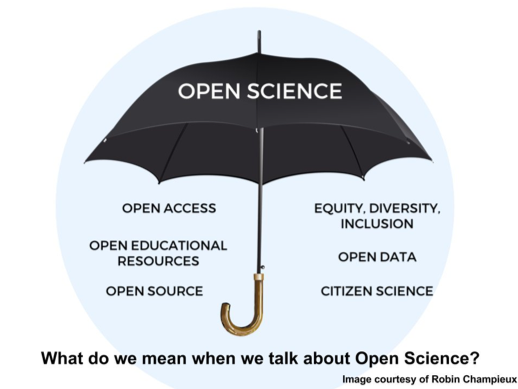
\includegraphics[scale=0.7]{open_science_eosc-hub}}
    \caption{Definition der Open Science-Handlungsfelder nach der Europäischen Kommission.\protect\footnotemark}
    \label{fig:openscience1}
\end{figure} \footnotetext{URL: \url{https://www.eosc-hub.eu/open-science-info} (letzter Zugriff am 03.05.2022).}

Die Europäische Kommission definiert für das große EU-Infrastrukturprojekt ,,European Open Science Cloud'' (EOSC)\footnote{Siehe Abschnitt ,,Infrastrukturen''.}, welche im Rahmen des Langzeitprogramms \textit{Horizon Europe} aufgebaut wird\footnote{Horizon Europe startete 2020 und läuft noch bis 2027 mit einem Förderungsumfang von insgesamt 95,5 Milliarden Euro (Phase 2021-27), URL: \url{https://ec.europa.eu/info/research-and-innovation/funding/funding-opportunities/funding-programmes-and-open-calls/horizon-europe_en} (letzter Zugriff am 03.05.2022)}, sechs Handlungsfelder - wie aus der Abbildung \ref{fig:openscience1} hervorgeht. Diese kombinieren im Kern Praktiken aus der traditionellen Wissenschaft mit den Open Science-Grundsätzen und entwickeln daraus schwerpunktartig Lösungskonzepte für die wissenschaftliche Forschung. Das Open Data-Konzept unter dem Dach der Open Science konzentriert sich auf den wissenschaftlichen Umgang mit den im Forschungsprozess anfallenden digitalen Forschungsdaten, während sich Open Access-Konzepte mit Fragen des freien Zugangs zu diesen und sonstigen wissenschaftlichen Materialen beschäftigen. Citizen Science-Konzepte entwickeln Lösungen, wie unter Beibehaltung wissenschaftlicher Integrität Partizipation in der Wissenschaft gestärkt werden kann.\footnote{Siehe zum Beispiel die Citizen Science-Plattform ,,Bürger schaffen Wissen'', URL: \url{https://www.buergerschaffenwissen.de/} (letzter Zugriff am 03.05.2022).}

\begin{figure}[h]
    \centering
    \frame{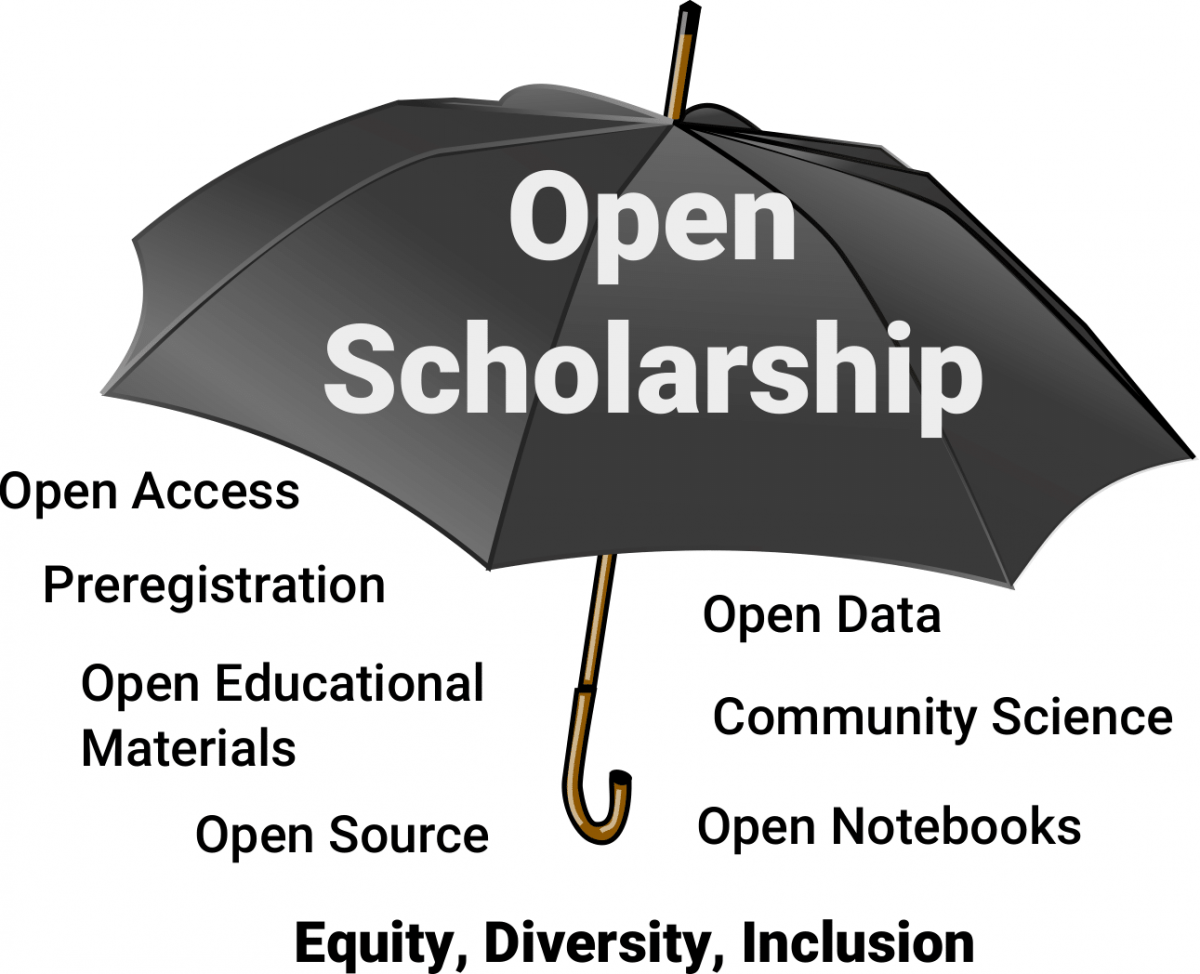
\includegraphics[scale=0.2]{open_science_british-psy-soc}}
    \caption{Definition der Open Science-Handlungsfelder (hier Open Scholarship) nach der Britischen Gesellschaft für Psychologie (The British Psychological Society).\protect\footnotemark}
    \label{fig:openscience2}
\end{figure} \footnotetext{URL: \url{https://thepsychologist.bps.org.uk/volume-33/november-2020/bropenscience-broken-science} (letzter Zugriff am 03.05.2022). Zu sehen ist hier auch die unterschiedliche Begriffsverwendungen ,,Open Science'' und ,,Open Scholarship''}

Die Handlungsfelder können voneinander abweichen, wie ein Blick auf die Abbildung \ref{fig:openscience2} zeigt. Die Abweichungen zwischen beiden Abbildungen lassen den Schluss zu, dass es letztlich vom konkreten (wissenschaftlichen) Kontext abhängt, welche Handlungsfelder unter Open Science definiert werden und es hier folglich eine strenge Vorgabe nicht gibt. Schließlich hängt diese Definition auch davon ab, wo und ob überhaupt Handlungsbedarf für Open Science gesehen wird. Dass die Replikationskrise dringenden Handlungsbedarf vorwiegend in den Lebens- und Naturwissenschaften offenbart hat, heißt nicht, dass dieser gleichermaßen auch in geisteswissenschaftlichen Fächern gesehen wird, wo vorwiegend hermeneutische Forschungsmethoden angewandt werden, die sich fundamental von den statistisch empirschen der Naturwissenschaften unterscheiden. Das bedeutet, dass Handlungsbedarf gegebenenfalls erst noch geschaffen werden muss. 

\paragraph{Infrastrukturen} Anhand der gegenwärtigen fachübergreifenden Anwendungsmöglichkeiten von Open Science in der eigenen Forschung können grob drei Gruppen von technischen Infrastrukuren unterschieden werden: 1. zentrale, 2. dezentrale und 3. nachgenutzte Infrastrukturen.

\begin{enumerate}
\item Begleitend zur Reproduzierbarkeitsstudie des COS wurde das \textit{Open Science Framework} (OSF)\footnote{URL: \url{https://osf.io/} (letzter Zugriff am 28.04.2022).} entwickelt, das im Hintergrund eine zentrale IT- Infrastruktur über eine Plattform bereitstellt, die bekannte Open Science-Verfahren wie Präregistrierung, Preprints und Generierung von Permalinks ermöglicht. Zum Funktionsumfang gehören außerdem Projektversionierung sowie ein generisches Repositorium zum Speichern und Aggregieren multipler Inhalte unterschiedlicher Formaten. Im veröffentlichten, diese Arbeit von Beginn an begleitenden, OSF-Projekt ,,Master thesis: Open Science in History?''\footnote{URL: \url{https://osf.io/sc9yf/?view_only=aa5eb53a48ba4eaab512d049712d704a}, hier nur mit lesendem Zugriff auf das Projekt.} wurde unter anderem die LaTex-Version der schriftlichen Arbeit, welche mit Git versioniert und auf GitHub zugänglich ist, und die Zotero-Library mit der verwendeten Literatur über die Add-ons-Funktionalität hinzugefügt. Heterogene Dienste und verteilte Ressourcen können also im OSF zusammengeführt und dort synchron gehalten werden. Damit ist das OSF im Kern ein Projektmanagement-Tool, das Wissenschaftler*innen dabei unterstützt, ihr methodisches Vorgehen transparent zu machen sowie Workflows zu automatisieren und dadurch systematisch Open Science über den gesamten Forschungsprozess zu praktizieren.\footnote{Vertrauensvorschuss erhält das COS vor allem durch eine konsequent transparente Politik wie zum Beispiel der Veröffentlichung aller Finanzberichte, URL: \url{https://www.cos.io/about/finances} (letzter Zugriff am 28.04.2022).} Dass das OSF steigende Anwenderzahlen insbesondere durch akademische Einrichtungen in den USA verzeichent,\footnote{Zum Beispiel Princeton University, New York University, George Washington University, u.a. Siehe \url{https://osf.io/institutions} (letzter Zugriff am 21.04.2022).}, weist darauf hin, dass es das Potential hat, sich zu einem Standard zu entwickeln.\footnote{Positiv hervorzuheben ist zudem, dass das COS alle seine Softwareprodukte auf GitHub in Open Source veröffentlicht. Siehe URL: \url{https://github.com/CenterForOpenScience} (letzter Zugriff am 30.04.2022).}

\item Eine andere Entwicklung ist derzeit auf europäischer Ebene zu beobachten, wo es ein zentrales und globales Infrastrukturangebot, wie das OSF, nicht gibt. Zwar existieren einzelne fachübergreifende Projekte wie zum Beispiel das Repositorium \textit{Zenodo} (seit 2016)\footnote{URL: \url{https://zenodo.org/} (letzter Zugriff am 28.04.2022)}, doch ist dieses Infrastrukturangebot funktional auf die Archivierung und Verfügbarmachung einzelner digitaler Ressourcen zugeschnitten\footnote{Siehe Upload-Seite in Zenodo, URL: \url{https://zenodo.org/deposit/new} (letzter Zugriff am 30.04.2022)}, die wiederum von ,,Communities'' kuratiert werden können\footnote{Zum Beispiel die Community ,,Deutsch-jüdische Geschichte'', URL: \url{https://zenodo.org/communities/djg} (letzter Zugriff am 28.04.2022)}. Auf die Masterarbeit angewandt, konnte das GitHub-Repositorium mit der Versionierung hier nicht - analog zum OSF - eingebunden und synchronisiert werden. Zenodo bietet die Möglichkeit, automatisiert den jeweils aktuellen Repo-Release von GitHub als verpackte .zip-Archivdatei hochzuladen und zu veröffentlichen.\footnote{Siehe URL: \url{https://zenodo.org/account/settings/github/} (letzter Zugriff am 28.04.2022)} Der erste Release dieser Arbeit erfolgte aber üblicherweise erst mit deren Abgabe und damit in der finalen Phase des Forschungsprozesses. Das ist kein Beleg, aber ein Indiz dafür, dass der Schwerpunkt in Zenodo auf \textit{publizierbaren} Ressourcen liegt. Diese Vermutung wird auch von einer Stichprobenauswertung zur Nutzung von Zenodo in dessen globaler Suche nach ,,Datasets'' und ,,Publications | Articles'' gestützt.\footnote{Dies kann über die Versionsnummer der Ressource identifiziert werden. URL der Suchanfrage am 29.04.2022: \url{https://zenodo.org/search?page=1&size=20&type=dataset&type=publication&subtype=article&sort=mostrecent} Die Mehrheit der Artikel und Datensätze existieren häufig nur in einer Version (v1), was dafür spricht, dass insbesondere die finalen Ergebnisse auf Zenodo archiviert werden. Es wäre an dieser Stelle interessant gewesen, einmal systematisch und mit computationalen Methoden zu evaluieren, wie Zenodo von Wissenschaftler*innen verwendet wird und empirisch gesicherte Aussagen zu treffen, wie Open Science gegenwärtig bereits praktiziert wird. Dies könnte zum Beispiel mit der von Zenodo bereitgestellten öffentlichen REST-API oder dem OAI-PMH Protokoll realisiert werden, URL: \url{https://developers.zenodo.org/} (letzter Zugriff am 29.04.20222). Diese Auswertung konnte im Rahmen der Arbeit nicht mehr geleistet werden.} Auf GitHub bezogen, besteht der Hauptunterschied zum OSF darin, dass Zenodo bis auf Releases keine Services zur Integration automatisierter Workflows im Portfolio hat, die in erster Linie eine arbeitsunterstützende Wirkung haben. Wer mit Zenodo konsequent Open Science phasenübergreifend praktizieren will, muss dies über aufwändigeres manuell iteratives Hochladen von Ressourcen machen. 

Mit der \textit{European Open Science Cloud} (EOSC, seit 2018)\footnote{URL: \url{https://eosc-portal.eu/} (letzter Zugriff am 27.04.2022)} gibt es aktuell ein größeres europäisches Infrastrukturprojekt, das zum Ziel hat, Dienste, Daten und andere Ressourcen ,,from a wide range of national, regional and institutional public research infrastructures across Europe''\footnote{Europäische Kommission (Hrsg.): European Open Science Cloud, URL: \url{https://digital-strategy.ec.europa.eu/en/policies/open-science-cloud} (letzter Zugriff am 28.04.2022).} über das \textit{EOSC Portal}\footnote{URL: \url{https://eosc-portal.eu/} (letzter Zugriff am 28.04.2022).} zentral zu verzeichnen, die wiederum von EOSC-Nutzer*innen in eigenen Projekten verwaltet werden können. Der Unterschied zum OSF besteht darin, dass die EOSC kein Infrastrukturangebot ist, auf der individuell Open Research praktiziert werden kann. Die EOSC ist selbst nur Aggregator bereits existierender Angebote, registriert und vernetzt diese miteinander. Sie ist mehr Verzeichnes als Plattform, das Sichtbarkeit und Recherchierbarkeit dezentraler Infrastrukturen ermöglicht. Die Interaktionsmöglichkeiten sind daher auf diese Zwecke beschränkt.\footnote{Auch hier wurde testweise ein Projekt für die Masterarbeit angelegt. Eigene Ressourcen konnten nicht hochgeladen/ eingebunden, sondern nur in der Cloud registrierte Open Science Angebote in einer privaten Liste gespeichert werden..}

\item Neben dem Aufbau neuer Infrastrukturen für die Wissenschaft gibt es außerdem den Ansatz, bestehende und etablierte Infrastrukturen aus der weiter gefassten Open-Bewegung nutzbar zu machen. Hervorzuheben sind die Angebote der Wikimedia Foundation, die sich, wie in Kapitel 2.1.1 beschrieben, mit dem ,,Fellow-Programm Freies Wissen'' bereits aktiv in Open Science eingebracht hat. Aktuell laufen unterschiedliche Projekte, die das sogenannte Wiki*versum in der wissenschaftlichen Forschungsarbeit nutzen. Aus dem Fellow Programm stammt das Wiki*versum-Projekt \textit{Die Datenlaube}, in dem das Massenblatt ,,Die Gartenlaube – Illustrirtes Familienblatt'' aus dem 19. Jahrhundert mittels Commons, Wikisource und Wikidata kollaborativ erschlossen und analysiert wurde.\footnote{In Commons digitalisiert (\url{https://commons.wikimedia.org/w/index.php?title=Category:Gartenlaube_(Magazine)&oldid=334192328&uselang=de}), mit Wikisource transkribiert (\url{https://de.wikisource.org/w/index.php?title=Die_Gartenlaube&oldid=4048963}) und in Wikidata strukturiert erfasst und ausgewertet. Siehe zum Projekt auch das öffentliche Repositorium auf GitHub, URL: \url{https://github.com/DieDatenlaube} sowie das Blog, URL: \url{http://diedatenlaube.github.io}. Ein Überblick über das Projekt ist auf das Wikimedia-Blog veröffentlicht, siehe Christopher Schwarzkopf: Hilfe für die Datenlaube: mit [[Wikisource+Wikidata]] die freie Quellensammlung verbessern, Wikimedia Deutschland, 16. Oktober 2019, URL: \url{https://blog.wikimedia.de/2019/10/16/hilfe-fuer-die-datenlaube-mit-wikisourcewikidata-die-freie-quellensammlung-verbessern/} (letzter Zugriff am 01.05.2022).} Ein weiteres, nicht aus dem Fellow Programm stammendes Projekt ist die \textit{Bamberger Islam-Enzyklopädie}. Bei diesem wurde wissenschaftlich betreut in der deutschsprachigen Wikipedia eine Enzyklopädie zum Themenbereich Islam aufgebaut und wird in der Fortsetzung kollaborativ ergänzt.\footnote{Siehe Vorstellung des Projekts auf der Website der Universität Bamberg, URL: \url{https://www.uni-bamberg.de/islamwissenschaft/bie/} (letzter Zugriff am 01.05.2022). Beispielartikel in der Wikipedia \textit{Fādilīya}, URL: \url{https://de.wikipedia.org/w/index.php?title=Fādilīya&oldid=202323908.}} Vorteilhaft bei den Wiki*versum-Lösungen ist die Ausnutzung von Synergieeffekten. Die Wissenschaft kann die langjährigen Erfahrungen der Wikimedia bei der technischen Implementierung von Offenheitskriterien für sich nutzen und deren Tools frei verwenden. Umgekehrt können dadurch gleichzeitig fundierte Erkenntnisse aus der wissenschaftlichen Forschung effizient in die Öffentlichkeit transferiert und das Wissen im Wiki*versum dadurch für alle verbessert werden. Die Projekte zeigen schließlich auch, dass vorhandene offene Infrastrukturen für die wissenschaftliche Forschung adaptiert und damit nutzbar gemacht werden können. Mit dem großen Angebotsspektrum bietet sich zudem für viele Open Sciene-Handlungsfelder eine Nutzungsoption. Auch wenn sich die WMF im Bereich der Open Science engagiert, bleibt alledings abschließend anzumerken, dass deren Angebote nicht auf die Bedürfnisse der Wissenschaft zugeschnitten sind, sondern in erster Linie dem Grundsatz des freien Wissens für alle folgen. Daher muss für jedes Projekt individuell evaluiert werden, inwiefern hier ein oder mehrere Wikimedia-Angebote für die eigene Forschungsarbeit in Frage kommen.\footnote{Dies wird auch in den beiden vorgestellten wissenschaftlichen Wiki*versum-Projekten kritisch reflektiert.}    
\end{enumerate}

Der Blick auf die Infrastrukturebene zeigt, dass die Möglichkeiten von offener Wissenschaft stark von den Infrastrukturen im Hintergrund abhängen. Letztendlich manifestiert sich in ihnen der Grad an Open Science, der am Ende von Forschenden praktiziert werden kann. Daher ist es nicht nur auf der Konzept-, sondern auch auf der Infrastrukturebene wichtig, Bedarfe und Standards für die wissenschaftliche Forschung zu formulieren. Seitens der Anbieter von Open Science-Infrastrukturen müssen diese Anforderungen aufgenommen und umgesetzt werden. Sie stehen hier in der Verantwortung, mögliche Machtgefälle und Abhängigkeiten fortlaufend zu reflektieren und zu kommunizieren, das heißt sich die Frage nach Vertrauenswürdigkeit und Legitimation immer wieder neu zu stellen. In diesem Zusammenhang wurden bereits die \textit{TRUST Principles} formuliert, die Transparency, Responsibility, User focus, Sustainability and Technology als Rahmenbedingungen bei der Infrastrukturentwicklung vorgeben.\footnote{Vgl. Dawei Lin, Jonathan Crabtree, Ingrid Dillo, u.a.: The TRUST Principles for digital repositories, in: Scientific Data, Ausgabe 144, 2020, S. 6ff., doi:10.1038/s41597-020-0486-7.}

\section{Forschungsdatenmanagement}

Die historischen Daten zu Jüdischen Gewerbebetrieben zeigen exemplarisch, dass digitale Forschungsdaten längst Bestandteil auch in der Forschungsarbeit von Historiker*innen geworden sind. Mit ihnen rücken in den Geschichtswissenschaften (neue) computergestützte qualitative wie quantitative Analyse- und Auswertungsverfahren in den Fokus.\footnote{Im Zuge dieser Entwicklung haben sich inzwischen Lehrstühle wie der für Digital History an der Humboldt-Universität zu Berlin etabliert, die sich auf ,,digitale Methoden, Techniken und Standards für die Geschichtswissenschaften'' sowie auf ,,den digitalen Transformationsprozess im Fach'' spezialisiert haben, URL: \url{https://www.geschichte.hu-berlin.de/de/bereiche-und-lehrstuehle/digital-history/profil} (letzter Zugriff am 03.05.2022).}

Wenn aber Forschungsdaten epistemologisch an Bedeutung für die Wissenschaft gewinnen, dann stellen sich unweigerlich Fragen nach dem wissenschaftlichen Umgang mit ihnen. Daraus wurde sowohl auf wissenschaftlicher als auch auf politischer Ebene bereits die Notwendigkeit eines nachhaltigen Forschungsdatenmanagements (FDM) abgeleitet, welches sich mit der Gestaltung wissenschaftlicher Standards, Workflows und Best Practices zur Handhabung von digitalen Forschungsdaten im Forschungsprozess und darüber hinaus auf methodischer, konzeptioneller, organisatorischer und technischer Ebene beschäftigt.\footnote{Vgl. Johannes Fournier: Komplexität und Vielfalt gestalten, in: Markus Putnings, Heike Neuroth, Janna Neumann (Hrsg.), Praxishandbuch Forschungsdatenmanagement, Berlin/Boston 2021, S. 3, doi:10.1515/9783110657807.} FDM will phasenübergreifende Qualität von Forschung auch im digitalen Zeitalter sicher stellen. Ziel ist zudem, Datentransfer und Datennutzung zu fördern. Damit knüpft FDM direkt an die Open Science-Grundsätze der Transparenz, Kollaboration und Wiederverwendbarkeit an, auch wenn es den ,,Openess''-Gedanken nicht im Namen trägt und als Konzept FAIR Data nutzt.\footnote{Siehe Kapitel 2.2.2.} sind die Anknüpfungspunkte an Open Science offentsichtlich, die sich auch in den \textit{FAIR Principles} manifestieren, die in Kapitel 2.2.2 näher erläutert sind. Von daher ist es naheliegend Forschungsdatenmanagement und Open Science zusammenzudenken, was im wissenschaftlichen Diskurs und in der Praxis bereits passiert.\footnote{So zum Beispiel im Zusammenhang mit der unter Kapitel 2.1.3. vorgestellten EOSC. Vgl hierzu Achim Streit und Jos van Wezel: Deutschland in der European Open Science Cloud, in: Praxishandbuch Forschungsdatenmanagement, 2021, S. 31-52. Am Helmholtz-Zentrum ist FDM direkt an das dortige Helmholtz Open Science Office angebunden. Siehe N. L. Weisweiler, R. Bertelmann, J. Bumberger, K. Elger, M. Fiedler, P. Fuhrmann, O. Knodel, R. Krahl, Ö. Özkan, F. Rhiem, I. Schmahl, S. Servan, A. Upmeier, K. Wedlich-Zachodin (2022): Helmholtz Open Science Briefing. Helmholtz Open Science Praxisforum Forschungsdatenmanagement: Report, (Helmholtz Open Science Briefing), Potsdam : Helmholtz Open Science Office, doi:10.48440/os.helmholtz.044. Auch im Open Science-Thesaurus des Institut de l’information scientifique et technique in Vandoeuvre-lès-Nancy (Frankreich) erscheint FDM, doi:10.13143/lotr.9297.}

Klar ist, dass die Aufgabe eines Forschungsdatenmanagements allein auf individueller Ebene nicht bewältigt werden kann, sondern dafür entsprechende Infrastrukturen und Dienste bereitgestellt werden müssen. Aktuell gibt es nationale Anstrengungen wie die ,,Nationale Forschungsdateninfrastruktur (NFDI)'' am Bundesministerium für Bildung und Forschung (BMBF), die in dieser offenen Situation die Entwicklung von Lösungsstrategien massiv fördern und vorantreiben wollen.\footnote{Nationale Forschungsdateninfrastruktur, BMBF, URL: \url{https://www.bmbf.de/de/nationale-forschungsdateninfrastruktur-8299.html (letzter Zugriff am 04.05.2022).}} Diese deutsche Initiative geht zurück auf die Bund-Länder-Vereinbarung zu Aufbau und Förderung einer Nationalen Forschungsdateninfrastruktur (NFDI) vom 26. November 2018, in der ein Förderzeitraum von 2019 bis 2028 und eine jährlich Fördersumme von 90 Millionen Euro für 30 Forschungsverbünde (sogenannte Konsortien) vorgesehen sind.\footnote{Bund-Länder-Vereinbarung zu Aufbau und Förderung einer Nationalen Forschungsdatenin-frastruktur (NFDI) vom 26. November 2018. URL: \url{https://www.gwk-bonn.de/fileadmin/Redaktion/Dokumente/Papers/NFDI.pdf} (letzter Zugriff am 04.05.2022).} Mit der Durchführung wurde die Deutsche Forschungsgemeinschaft (DFG) beauftragt.\footnote{Nationale Forschungsdateninfrastruktur, DFG, URL: \url{https://www.dfg.de/foerderung/programme/nfdi/} (letzter Zugriff am 04.05.2022).} Zur organisatorischen Koordination auf der wissenschaftlichen Ebene hat sich 2020 der Verein Nationale Forschungsdateninfrastruktur (NFDI) e.V. gegründet.\footnote{URL: \url{https://www.nfdi.de/verein/} (letzter Zugriff am 04.05.2022).} Aus der aktuell veröffentlichten statistischen Übersicht der DFG geht hervor, dass in der dritten Antragsrunde, die zum Zeitpunkt des Verfassens dieser Arbeit noch lief, auch geschichtswissenschaftlich arbeitende Fachdisziplinen mit dem Titel ,,NFDI4Memory - Konsortium für historisch arbeitende Geisteswissenschaften'' vertreten sind.\footnote{DFG (Hrsg.): Nationale Forschungsdateninfrastruktur. Statistische Übersichten zum Antragseingang (Dritte Ausschreibungsrunde, November 2021), Stand: 26.11.2021, Version: 1.0, S. 18, URL: \url{https://www.dfg.de/download/pdf/foerderung/programme/nfdi/statistik_antragseingang_nfdi_3_runde_20211202.pdf} (letzter Zugriff am 04.05.2022).} Zudem ist seit 2019 die Website \url{https://4memory.de/} online, auf der zum Vorhaben und über aktuelle Aktivitäten informiert wird. Auch der \textit{Verband der Historiker und Historikerinnen in Deutschland} (VHD) engagiert sich in NFDI4Memory\footnote{Siehe VHD (Hrsg.): Geschichtswissenschaft im digitalen Zeitalter: NFDI4Memory, veröffentlicht am 10.09.2019, URL: \url{https://www.historikerverband.de//verband/nfdi.html} (letzter Zugriff am 04.05.2022).}, das - sollte es positiv beschieden werden - voraussichtlich im Januar 2023 an den Start gehen könnte.\footnote{Vgl. DFG (Hrsg.): Zeitplan für das Entscheidungsverfahren zur Förderung von Basisdiensten in der Nationalen Forschungsdateninfrastruktur, Stand 7. Dezember 2021, URL: \url{https://www.dfg.de/download/pdf/foerderung/programme/nfdi/zeitplan_nfdi_basisdienste_20211208.pdf} (letzter Zugriff am 05.05.2022).}

Festzuhalten bleibt abschließend, dass Handlungsbedarf für Forschungsdatenmanagement mehrheitlich auf allen Eben erkannt und die Weichen zur Umsetzung von FDM gestellt wurden. Deutlich geworden ist jedoch auch, dass sich die notwendigen Infrastrukturen dafür gegenwärtig noch im Aufbau befinden.   

\subsection{Forschungsdaten und Forschungsdatenlebenszyklus}

Gegenstand von Forschungsdatenmanagement sind Forschungsdaten. Generell sind damit digitale Ressourcen gemeint, die im Zuge wissenschaftlicher Forschungsarbeit erzeugt werden. Aber nicht alle Daten aus dem Forschungsprozess sind Forschungsdaten. Als Abgrenzungskriterium gilt, dass Forschungsdaten Grundlage von Forschungsergebnissen sind, also einen epistemologischen Wert  für die wissenschaftliche Forschung haben. Welche Daten genau darunter fallen, ist in jedem Forschungsvorhaben indiviuell zu definieren.\footnote{Vgl. S. Blumesberger (2021): Forschungsdaten in den Geisteswissenschaften. Bereits selbstverständlich oder doch noch etwas exotisch?, O-Bib. Das Offene Bibliotheksjournal / Herausgeber VDB, 8(4), S. 1–8, doi:10.5282/o-bib/5739.} Im Zusammenhang mit dieser Arbeit sind die Audiodateien der Experteninterviews, die zugehörigen Transkripte und das Codesystem eindeutig als Forschungsdaten zu definieren, wohingegen die E-Mail-Nachrichten mit den Terminabsprachen für die Interviews nicht darunter gezählt werden würden, da sie für die Erkenntnisgenerierung nicht relevant waren. Das bedeutet aber nicht, dass E-Mails per se keine Forschungsdaten sein können. Wie nun schon mehrfach festgestellt, ist diese Einstufung kontextabhängig.

Forschungsdaten durchlaufen in der Regel einen mehrstufigen Prozess. Um eine wissenschaftlich korrekte Handhabung in jeder Forschungsphase zu garantieren, orientiert sich FDM an einem idealtypischen Forschungsdatenlebenszyklus (Abb. 2.3).

\begin{figure}[h]
    \centering
    \frame{\includegraphics[scale=0.8]{datenlebenszyklus_forschungsdaten-info.png}}
    \caption{Idealtypischer Forschungsdatenlebenszyklus\protect\footnotemark}
    \label{fig:x cubed graph}
\end{figure} \footnotetext{URL: \url{https://www.forschungsdaten.info/themen/informieren-und-planen/datenlebenszyklus/}, Public Domain, (letzter Zugriff am 05.05.2022)}

An sich hält dieser Zyklus keine fundamental neue Information für die Wissenschaft bereit. Vor allem die ersten vier Phasen entsprechen den vertrauten und etablierten Phasen im Forschungsprozess. Neu hingegen sind die letzten zwei Phasen der Datenarchivierung und -nachnutzung, denn hier geht FDM über den traditionellen Forschungsprozess hinaus. Forschungsdaten sollen über die Laufzeit von Forschungsprojekten hinaus langfristig verfügbar und nachnutzbar gehalten werden, sodass sie Ausgangspunkt wieder neuer Forschungsvorhaben sein können. Dieses ,,Zurückspielen'' in den Forschungsprozess als iterativer Vorgang stellt ein zentrales Merkmal von Forschungsdatenmanagement dar.

\subsection{FAIR und Open Data}

Qualitätskriterien zum wissenschaftlichen Umgang mit Forschungsdaten werden im FDM durch die \textit{\textbf{F}(indable)\textbf{A}(ccessible)\textbf{I}(nteroperable)\textbf{R}(e-usable) Principles} definiert. Sie wurden im Jahr 2016 erstmals veröffentlicht\footnote{Siehe M. Wilkinson, M. Dumontier, I. Aalbersberg, u.a.: The FAIR Guiding Principles for scientific data management and stewardship. Sci Data 3, 160018 (2016). https://doi.org/10.1038/sdata.2016.18.} und gehen auf einen Workshop des \textit{Lorentz Workshop Centers} an der Universität Leiden (Niederlande) aus dem Jahr 2014 zurück.\footnote{Vgl. The Future of Research Communications and e-Scholarship (FORCE 11), The FAIR Data Principles, URL: \url{https://force11.org/info/the-fair-data-principles/} (letzter Zugriff am 06.05.2022).} Die FAIR Data Principles haben sich seitdem zu einem Best Practice im Umgang mit Forschungsdaten in der Wissenschaft entwickelt. Zentral bei deren Umsetzung sind sogenannte Metadaten, welche die inhaltlichen Daten formal beschreiben (Daten über Daten). Sie sind insofern wichtig, als dass sie erstens den inhaltlichen Daten den notwendigen Kontext für eine nachträgliche Quellenkritik geben und zweitens den Ausgangspunkt zur Auffindbarkeit und Interoperabilität der inhaltlichen Daten bilden. Auch wenn diese selbst nicht veröffentlicht sind, erhöhen Metadaten insgesamt die Sichtbarkeit von Forschungsergebnissen. 

Wie FAIR Data technisch umgesetzt wird, ist in der Literatur und in anderen (digitalen) Formaten inzwischen hinreichend besprochen worden und wird im Rahmen dieser Arbeit daher nicht im Einzelnen wiederholt. Stattdessen wird auf die bereits existenten Informationsplattformen zu Forschungsdatenmanagement verwiesen, die auch in dieser Arbeit genutzt wurden: Im deutschsprachigen Raum ist vor allem das Portal forschungsdaten.info hervorzuheben, das an der Universität Koblenz gehosted wird\footnote{Bis März 2019 am Helmholtz-Zentrum Potsdam, Deutsches GeoForschungsZentrum GFZ, URL: \url{https://www.forschungsdaten.info/} (letzter Zugriff am 05.05.2022).} sowie auf das öffentliche Wiki forschungsdaten.org\footnote{Ebenfalls von der Uni Koblenz betrieben, URL: \url{https://www.forschungsdaten.org/index.php/Hauptseite} (letzter Zugriff am 05.05.2022).}. Auf internationaler Ebene gibt es die \textit{GO Fair Initiative} sowie das Institut \textit{The Future of Research Communications and e-Scholarship} (USA), welche jeweils ebenfalls eine ausführliche Informationsplattformen zur Implementierung von FAIR Data Grundsätzen bereitstellen.\footnote{Go Fair, URL: \url{https://www.go-fair.org/} und FORCE11, Guiding Principles for Findable, Accessible, Interoperable and Re-usable Data Publishing version b1.0, URL: \url{https://force11.org/info/guiding-principles-for-findable-accessible-interoperable-and-re-usable-data-publishing-version-b1-0/}(alle letzter Zugriff am 05.05.2022).} Ziel dieser Angebotsformate ist es, praxisnah und für unterschiedliche Wissenschaftsbereiche FDM und FAIR Data zu vermitteln.\footnote{Wie wichtig diese Form der Wissenschaftskommunikation und Vermittlung ist, macht auch die aktuelle Ankündigung der DFG ,,Aktualisierung des Förderprogramms Informationsinfrastrukturen für Forschungsdaten'' deutlich, in der ,,umfangreichen Maßnahmen zu Aufbau und Weiterentwicklung von Informationsinfrastrukturen für Forschungsdaten'' geplant sind, Information für die Wissenschaft Nr. 32 vom 3. Mai 2022, URl: \url{https://www.dfg.de/foerderung/info_wissenschaft/info_wissenschaft_22_32/} (letzter Zugriff am 05.05.2022).}

Interessanter ist im Rahmen dieser Arbeit die Frage, in welchem Verhältnis das Konzept FAIR Data zu Open Data steht. Denn wie in Kapitel 2.1.3 gezeigt wurde, rekurriert Open Science nicht auf FAIR sondern auf Open Data als Lösungskonzept. Welcher Unterschied besteht also zwischen beiden Konzepten beziehungsweise warum ist es notwendig, neben Open Data, auch noch FAIR Data zu formulieren. Und die entscheidenede Frage ist: Sind die FAIR Data Principles Open Science? 

Für einen Abgrenzungsversuch werden zwei Kerneigenschaften von Open Data herangezogen. Erstens steht bei Open Data Interoperabiltät von Daten im Zentrum. Damit verbunden ist die Hoffnung, dass durch Austausch und Teilen konsequent offener Daten, Datensätze gänzlich neu kombiniert, aggregiert oder verknüpft werden können, woraus wiederum neue offene Werke jeglicher Art geschaffen werden können.\footnote{Vgl. ebd.} Hierin wird das Innovationspotential von Open Data gesehen. Neben offener Lizenzierung ist Voraussetzung dafür, dass die Daten in einem offenen Format vorliegen, welche nach dem 5-Sterne-Modell des WWW-Erfinders und Linked Open Data-Initiators Tim Berners-Lee klassifiziert sind.\footnote{URL: \url{https://5stardata.info/en/} (letzter Zugriff am 06.05.2022).} Diese Modell gibt zum einen eine basale Orientierung darüber, welche Formate als ,,offen'' gelten. Darunter werden vor allem nicht-proprietäre Formate gezählt. Gleichzeitig bildet es eine Abstufung und repräsentiert damit die möglichen Open Data-Grade. Im höchsten Grad (= 5 Sterne) können Daten aus dezentralen Datenquellen im gesamten Web maschinell identifiziert und verknüpft werden. Dieses Konzept wird als \textit{Linked (Open) Data} bezeichnet und ermöglicht, nicht mehr nur Daten, sondern Informationen maschinell zu verarbeiten.\footnote{Vgl. Tim Berner-Lee: Linked Data, digitales Paper veröffentlicht am 27.07.2006, URL: \url{https://www.w3.org/DesignIssues/LinkedData.html} (letzter Zugriff am 06.05.2022). Siehe auch Günther Neher, Bernd Ritschel: Semantische Vernetzung von Forschungsdaten, in: Stephan Büttner, Hans-Christoph Hobohm, Lars Müller (Hrsg.), Handbuch Forschungsdatenmanagement, Bad Honnef 2011, S. 169-190.} Die Vision dahinter ist, vom ursprünglichen Web of Documents, über ein Web of Data hin zu einem Web of Linked Data oder auch Semantic Web zu kommen, mit Wissen digital abgebildet, gespeichert und abgefragt werden kann.\footnote{Siehe Informationsportal des WWW-Konsortium (w3c) zum Semantic Web, URL: \url{https://www.w3.org/standards/semanticweb/} (letzter Zugriff am 06.05.2022).} Die in FAIR Data separat formulierten Kriterien der Auffindbarkeit, Zugänglichkeit und Wiederverwendbarkeit von Daten werden bei Open Data vorausgesetzt, um in der höchsten Stufe Interoperabilität zu erreichen. Allerdings können Daten, die nicht interoperabel sind, nach dem 5-Sterne-Modell trotzdem Open Data sein, wenn sie zum Beispiel als PDF- (= 1 Stern) oder CSV-Files (= 2 Sterne) vorliegen. Diese Variabilität lassen die FAIR Data Principles an dieser Stelle nicht zu. Hier reicht es zumindest in der Theorie streng genommen nicht aus, wenn (Meta)Daten in Form eines PDF's oder einer CSV für andere zugänglich aber nicht gleichzeitig interoperabel sind. Zu beachten ist daher, dass Forschungsdaten Open Data sein können ohne dabei die Grundsätze von FAIR Data zu erfüllen.

Zweitens geht Open Data im Allgemeinen über Open Access hinaus, zielt also nicht nur darauf ab, freien (lesenden) Zugang zu Daten zu schaffen, sondern dass diese gleichzeitig universell geteilt, modifiziert und neu publiziert werden können. Das setzt eine offene Lizenz der Daten voraus, wie sie in der ,,Open Definition'' der Open Knowledge Foundation eingefordert wird:

\begin{quote}
,,The work must be in the public domain or provided under an open license [...]. Any additional terms accompanying the work (such as a terms of use, or patents held by the licensor) must not contradict the work’s public domain status or terms of the license.''\footnote{Open Knowledge Open Definition Group: Open Definition. DEFINING OPEN IN OPEN DATA, OPEN CONTENT AND OPEN KNOWLEDGE, Version 2.1, URL: \url{https://opendefinition.org/od/2.1/en/} (letzter Zugriff am 06.05.2022).}
\end{quote}

Unter offener Lizenz wird demnach in erster Linie die Veröffentlichung ohne jegliche Restriktionen oder sonstige Vorgaben verstanden. Dies entspricht einer Veröffentlichung in Public Domain (CC0 ,,No Rights Reserved'')\footnote{Vgl. Creative Commons, URL: \url{https://creativecommons.org/share-your-work/public-domain/} (letzter Zugriff am 18.05.2022).}. Als ,,offen'' gelten auch jene Lizenzen, die als einzige Einschränkung die Namensnennung haben, aber die freie Nutzung von Daten erlauben (CC-BY und CC-BY-SA). Alle Lizenzen, welche die Nachnutzung in irgendeiner Form einschränken, zählen nach der OKF nicht mehr zu Open Data. 

Einen Standard für offene Lizenzen einzuführen, war und ist das Hauptanliegen des globalen Netzwerks \textit{Creative Commons} (CC).\footnote{URL: \url{https://creativecommons.org/} (letzter Zugriff am 18.05.2022).} Mit den \textit{Creative Commons licenses} stellt es allgemeingültige Lizenzen zur Verfügung, die für eigene Inhalte verwendet werden können.\footnote{Diese Arbeit zum Beispiel wurde in einer CC-BY-SA Lizenz auf GitHub veröffentlicht, siehe URL: \url{https://github.com/sopheck/offenes-fdm-fuer-historische-fd} (letzter Zugriff am 18.05.2022).} Anders als die OKF wird in der Frage der Offenheit eine Abstufung vorgenommen und ,,Most Open'' als \textit{Free Cultural Works}\footnote{Definition vom 17.02.2015, Version 1.1, URL (stable): \url{https://freedomdefined.org/index.php?title=Definition&oldid=19268} } kategorisiert, die mit Open Data gleichgesetzt werden können.\footnote{URL: \url{https://creativecommons.org/share-your-work/public-domain/freeworks} (letzter Zugriff am 18.05.2022).} Es werden jedoch auch wesentlich limitiertere Lizenzen zur Verfügung gestellt. Damit verfolgt die CC vor allem das Ziel, die ,,all rights reserved''-Lizenz, die jegliche  Nachnutzung von vornherein ausschließt, vermeidbar zu machen und Lizenzgeber zu ermutigen, frei lizensierbare Inhalte eindeutig zu kommunizieren.\footnote{Vgl. Creative Commons (2022): Understanding Free Cultural Works, URL: \url{https://creativecommons.org/share-your-work/public-domain/freeworks} (letzter Zugriff am 18.05.2022).}

Open Data ist demnach mit seiner Kultur der offene Lizensierung radikaler. Damit verfolgt die Open-Bewegung vor allem auch ein politisches Ziel. Aus steuerlich finanzierten Mitteln entstandene Daten aus dem öffentlichen Sektor (Wetter-, Verkehrs- oder Geodaten) sollen als Allgemeingut anerkannt und in der Konsequenz die Grundsatzziele der Partizipation und Bürgerbeteiligung als Paradigma in der Politik ausgestaltet werden.\footnote{Immerhin hat die aktuelle Regierungskoalition der BRD allgemein einen Rechtsanspruch auf Open Data zum Ziel erklärt, dessen unkonkrete Umsetzungsziele aber von der Wikimedia Deutschland kritisiert werden. Vgl. John Weitzmann, 
Justus Dreyling: Rechtsanspruch auf Open Data. Jetzt muss es endlich losgehen, Blogbeitrag auf Wikimedia Deutschland vom 17. März 2022, URL: \url{https://blog.wikimedia.de/} (letzter Zugriff am 06.05.2022).} Die Open-Bewegung stellt klar, dass darunter personenbezogene Daten nicht gezählt werden:

\begin{quote}
,,The key point is that when opening up data, the focus is on non-personal data, that is, data which does not contain information about specific individuals.''\footnote{Open Data Handbook der OKF: What is Open Data? Abschnitt What Data are You Talking About?, URL: \url{http://opendatahandbook.org/guide/de/what-is-open-data/} (letzter Zugriff am 06.05.2022).}
\end{quote} 

Hervorzuheben ist also, dass es ausschließlich um rechtlich unbedenkliche Daten geht, die in der Vergangenheit kaum oder gar nicht zugänglich waren und deren Öffnung Open Data vorantreiben will. Folgt man dieser Argumentation weiter, müssten demnach auch alle Forschungsdaten, die aus öffentlich finanzierten Forschungsprojekten stammen, in offener Lizenz veröffentlicht werden. Hier wiederum sind es die FAIR Data Principles, die in der Lizenzfrage Spielraum lassen und dazu explizit keine Vorgabe machen. Denn aus Sicht der Wissenschaft ist es möglich, dass forschungsethische Abwägungen oder eine eventuelle Gefährdung der wissenschaftlichen Integrität die Veröffentlichung von Forschungsdaten in einer Open Data-Form nicht erlauben.\footnote{Hierzu gehören in erster Linie sensible Daten in der Gesundheitsforschung. Vgl. FAIR4Health Consortium (Hrsg.): Improving Health Research in EU through FAIR Data, D2.3. Guidelines for implementing FAIR Open Data policy in health research.pdf, Version 1, 2019, URL: \url{https://osf.io/3u7dt/}.} Daher hat sich bei den FAIR Data Principles die Regel durchgesetzt, Daten ,,so eingeschränkt wie nötig und so offen wie möglich'' zu halten. Damit können Forschungsdaten, deren Zugriff auf eine exklusive Gruppe oder Domäne beschränkt ist, die FAIR Data Grundsätze vollumfänglich erfüllen und gleichzeitig niemals Open Data sein. Dennoch kann diese Praxis zu Open Science gezählt werden, da FAIR Data grundsätzlich wissenschaftliche Forschung öffnet, auch wenn dies nur für eine fest definierte Gruppe gilt. Aber auch in der Wissenschaft ist ein Trend zu Open Data erkennbar. Mit den \textit{Pantom Principles}, welche von der Open Knowledge Foundation in Zusammenarbeit mit Wissenschaftlern aus den USA und der UK initiiert wurden, soll in der Wissenschaft dafür sensibiliert werden, Open Data systematisch auch in der wissenschaftlichen Kontext mitzudenken.\footnote{Peter Murray-Rust, Cameron Neylon, Rufus Pollock, John Wilbanks: Panton Principles, Principles for open data in science, veröffentlicht am 19 Februar 2010, URL: \url{https://pantonprinciples.org/} (letzter Zugriff am 06.05.2022). Es handelt sich dabei nicht wie bei den FAIR Data Principles um handfeste Kriterien, sondern um Empfehlungen.} 

Dieser Gedanke soll in der in dieser Arbeit aufgegriffen und eine Strategie der Open Research Data verfolgt werden, die die Konzepte FAIR und Open Data kombiniert.\footnote{Diese Strategie wird auch von der Europäischen Komission empfohlen, siehe European Commission, Directorate General for Research and Innovation, Directorate B – Open Innovation and Open Science Unit B2 – Open Science (Hrsg.): Turning FAIR into reality. Final Report and Action Plan from the European Commission Expert Group on FAIR Data, Brüssel 2018, S. 21, doi:10.2777/1524.}